\documentclass[a4paper, 14pt,russian]{extarticle}

\usepackage[russian]{babel}
\usepackage[T2A]{fontenc}
\usepackage[utf8]{inputenc}
%Соответствующий математический шрифт для Times new roman
\usepackage{newtxmath}
\usepackage{fontspec} 
\usepackage{multirow}
%\usepackage{polyglossia}
%Times new roman
\defaultfontfeatures{Ligatures={TeX},Renderer=Basic} 
\setmainfont[Ligatures={TeX,Historic}]{Times New Roman}
\setmainfont{Times New Roman}
\setsansfont{Arial}
\setmonofont{Courier New}
\newfontfamily\cyrillicfont[Script=Cyrillic]{Times New Roman}
\newfontfamily\cyrillicfontsf[Script=Cyrillic]{Arial}
\newfontfamily\cyrillicfonttt[Script=Cyrillic]{Courier New}

%\setdefaultlanguage{russian}

%Геометрия
\usepackage{geometry}
\geometry{top=20mm}
\geometry{bottom=15mm}
\geometry{left=20mm}
\geometry{right=15mm}
\usepackage{setspace}
%Нормальные дроби через запятую
\usepackage{ncccomma}

\newcommand{\changefont}{%
	\fontsize{12}{11}\selectfont
}

%Заголовки
\usepackage{fancyhdr}
\pagestyle{fancy}
\fancyhf{}
%\renewcommand{\sectionmark}[1]{\markright{#1}}
\fancyhead[R]{\changefont \slshape \leftmark}
\fancyhead[L]{\changefont \slshape \rightmark}
%\newcommand{\ssubsection}[1]{\subsection*{#1}
%	\addcontentsline{toc}{subsection}{#1}
%	\markright{#1}{}}
\cfoot{\thepage}

%\полуторный интервал
\setstretch{1.15}
\setlength{\parindent}{1.25cm}

\usepackage{amsmath, amsfonts, mathtools}
\usepackage{physics}
\usepackage{indentfirst}
\usepackage{xcolor}
\usepackage{alltt}
\usepackage{graphicx}
\usepackage{wrapfig}
\usepackage{pgfplots}
\usepackage{filecontents}

%Настройка ссылок
\usepackage{hyperref}
%\usepackage{upgreek}
%\renewcommand{\beta}{\upbeta}
\hypersetup{
	colorlinks,
	citecolor=black,
	filecolor=black,
	linkcolor=black,
	urlcolor=black
}
\usepackage{caption}
\DeclareCaptionLabelSeparator{dot}{. }
\captionsetup{justification=centering,labelsep=dot}
\usepackage{titlesec}

%Формат заголовков
\titleformat{\section}{\bfseries\filcenter\Large}{\thesection}{1em}{}
\titleformat{\subsection}{\bfseries\filcenter\large}{\thesubsection}{1em}{}
\titleformat{\subsubsection}{\bfseries\filcenter\normalsize}{\thesubsubsection}{1em}{}

\usepackage{chngcntr}

%Включить в нумерацию картинок раздел
\counterwithin{figure}{section}

%Листинги кода и их стили
\usepackage{listings}
\usepackage{minted}
\lstdefinestyle{c++} {
	language=C++,
	breaklines=true,
	frame=single,
	numbers=left,
	basicstyle=\footnotesize\ttfamily,
	keywordstyle=\bfseries\color{green!40!black},
	commentstyle=\itshape\color{purple!40!black},
	identifierstyle=\color{blue},
	backgroundcolor=\color{gray!10!white},
}

\lstdefinestyle{python}{
	language=Python,
	breaklines=true,
	frame=single,
	numbers=left,
	keywordstyle=\bfseries\color{green!40!black},
	frame=lines,
	basicstyle=\footnotesize\rmfamily
}

\lstdefinestyle{cmd}{
	breaklines=true,
	frame=single,
	basicstyle=\footnotesize\ttfamily,
	frame=lines
	basicstyle=\footnotesize
}
\usepackage{tikz}
\usepackage{tkz-base}
\usetikzlibrary{quotes,angles}
\usetikzlibrary {arrows.meta}
%\usepackage{tkz-euclide}
\usetikzlibrary{calc}
\usetikzlibrary{shapes.geometric, shapes.misc, arrows}

\tikzstyle{startstop} = [rectangle, rounded corners, 
minimum width=3cm, 
minimum height=1cm,
text centered, 
draw=black]

\tikzstyle{io} = [trapezium, 
trapezium stretches=true, % A later addition
trapezium left angle=70, 
trapezium right angle=110, 
minimum width=3cm, 
minimum height=1cm, text centered, 
draw=black]

\tikzstyle{process} = [rectangle, 
minimum width=3cm, 
minimum height=1cm, 
text centered, 
text width=5cm, 
draw=black]

\tikzstyle{decision} = [diamond, 
minimum width=3cm, 
minimum height=1cm, 
text centered, 
draw=black]

\tikzstyle{startfor} = [chamfered rectangle, 
chamfered rectangle corners={north west, north east},
minimum width=3cm, 
minimum height=1cm, 
text centered, 
draw=black]

\tikzstyle{endfor} = [chamfered rectangle, 
chamfered rectangle corners={south west, south east},
minimum width=3cm, 
minimum height=1cm, 
text centered, 
draw=black]

\tikzstyle{block} = [style=draw, 
	minimum width = 1.6cm,
	minimum height = 1.2cm]
\tikzstyle{arrow} =[-{Latex[length=3mm]}, thick]

\newcommand{\drawsum}[2]{\node[draw,
	circle,
	minimum size=1cm
	] (#1) at #2{};
	\draw (#1.north east) -- (#1.south west)
	(#1.north west) -- (#1.south east)}

\newcommand{\fillsumsouth}[1]{\draw[fill=black] (#1.center) -- ++(-135:0.5cm) arc (-135:-45:0.5cm) -- cycle}
\newcommand{\fillsumnorth}[1]{\draw[fill=black] (#1.center) -- ++(135:0.5cm) arc (135:45:0.5cm) -- cycle}

\newcommand{\drawIIE}[2]{\node (#1)[draw, 
	minimum width = 1.6cm,
	minimum height = 1.2cm] at #2 {};   
	\draw [thick] ($(#1.west) + (0.3cm,-0.4cm)$) -- ($(#1.east) + (-0.3cm, -0.4cm)$);
	\draw [arrow] ($ (#1.center) + (0, -0.4cm) $) -- ($ (#1.north) + (0, -0.1cm) $);}

\begin{document}
	
	\begin{titlepage}
	\newpage
	\begin{center}
		
\includegraphics[width=\textwidth]{png/tit.png}
		Институт информационных и вычислительных технологий \\
			Кафедра управления и интеллектуальных технологий
		\vspace{1.25cm}
	\end{center}
	
	\vspace{1.2em}
	
	\begin{center}
		%\textsc{\textbf{}}
		\begin{spacing}{1}
			{\Large Отчёт по лабораторной работе №2 \linebreak
			По дисциплине <<Нейро-нечёткие технологии в задачах управления>> \\}
			\large{\bf<<Основы генетических алгоритмов>>}
		\end{spacing}
	\end{center}
	
	\vspace{5em}
	

	\vspace{6em}
	
		\noindent Выполнили студенты: Михайловский М., Томчук В. \\
		Группа: А-03-21 \\
		Бригада: 1\\
		Проверил: Косинский М.\,Ю.
	
	
	\vspace{\fill}
	
	\begin{center}
		Москва 2024
	\end{center}
	
\end{titlepage}
	\pagenumbering{arabic}
	\setcounter{page}{2}
	\tableofcontents
	\newpage
	
	\newcommand{\diag}[1]{\mathrm{diag}\,#1}
	\renewcommand{\sp}[1]{\mathrm{sp}\,#1}

	\section{Постановка задачи}
	
	Дана функция $f(x) = 2x^2 + 1$, необходимо найти её максимум с точностью до целого значения $x\in [0,\,15
	]$ с применением генетического алгоритма. График целевой функции $f(x)$ представлен на рис. \ref{graph}.
	
	\begin{figure}[h]
		\centering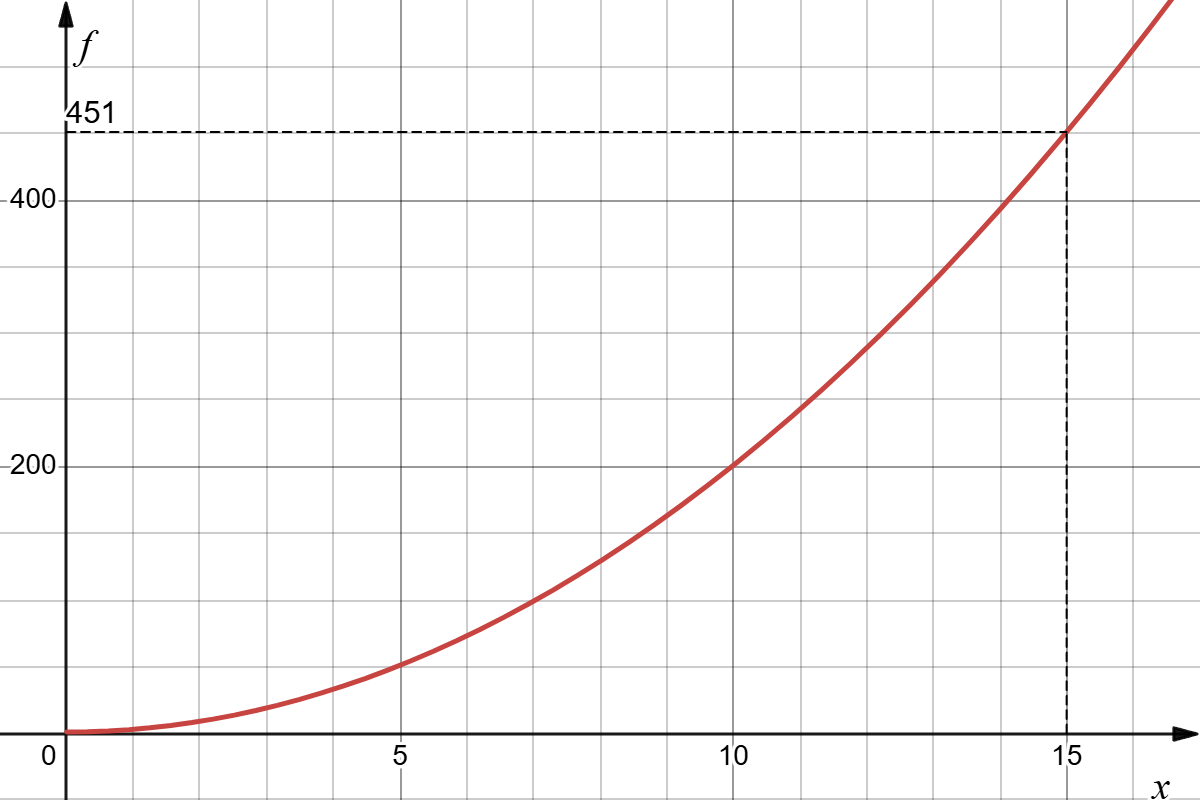
\includegraphics[width=.6\textwidth]{png/graph.png}
		\caption{График целевой функции}
		\label{graph}
	\end{figure}
	
	В рамках работы генетического алгоритма ищется такой генетический код $x_2 \equiv x$, такой что, функция приспособленности для него максимальна: ${f(x)\to\max}$. Здесь $x_2$ является бинарным представлением $x\in \mathbb{R}$.
	
	\section{Описание генетического алгоритма}
	
	Алгоритм имеет следующий вид (изначальная популяция особей уже выбрана и представлена в бинарном коде, изначальная приспособленность рассчитана):
	\begin{enumerate}
		\item Селекция особей для скрещивания;
		\item Мутация особей;
		\item Получение новой популяции в результате скрещивания;
		\item Расчёт приспособленности полученных особей;
		\item Проверка критерия остановки.
	\end{enumerate}

	\subsection{Селекция}
	
	В ходе работы было реализовано два метода селекции: классический и ранговый. Они определяют то, как из популяции размером $N$ выбираются особи для скрещивания.
	
	\textbf{Классический}. Для каждой $i$-ой особи рассчитывается относительная приспособленность:
	\begin{equation}
		f_\text{отн}(x_i) = \frac{f(x_i)}{\sum_{k=1}^N f(x_k)}
		\label{f_otn}
	\end{equation}

	Разыгрывается так называемая <<рулетка>>. По сути с помощью случайной величины $\xi \sim R(0, 1)$ выбирается особь для скрещивания. Вся область определения случайной величины $\xi$ делится и ставится в соответствие каждой особи, при чем величина сопоставляемого интервала соответствует относительной приспособленности $f_\text{отн}(x_i)$ этой особи.
	
	\begin{center}
		\begin{tikzpicture}
		\node (circ)[draw,
		circle,
		minimum size=6cm] at (0,0) {};
		\draw[fill=black] (circ.center) -- ++(-30:3cm);
		\draw[fill=black] (circ.center) -- ++(-130:3cm);
		\draw[fill=black] (circ.center) -- ++(-200:3cm);				
		\draw[fill=black] (circ.center) -- ++(90:3cm);	
		\node [] at (15:1.5cm) {$f_\text{отн}(x_1)$};	
		\node [] at (-80:1.5cm) {$f_\text{отн}(x_2)$};	
		\node [] at (-170:1.5cm) {$f_\text{отн}(x_3)$};	
		\node [] at (135:1.5cm) {$f_\text{отн}(x_4)$};
		\node [above right] at (0,3cm) {$0$};										
		\node [right] at (3cm,0) {$0,25$};
		\node [below] at (0,-3cm) {$0,5$};
		\node [left] at (-3cm,0) {$0,75$};
		\node [above left] at (0,3cm) {$1$};
		\end{tikzpicture}		
		\captionof{figure}{Распределение области определения $\xi$ в соответствии с относительными приспособленностями особей}
		\label{ruletka}
	\end{center}

	\textbf{Ранговый}. Для каждой особи рассчитывается относительная приспособленность в соответствии с формулой (\ref{f_otn}). Всей популяции в соответствии в зависимости от величины относительной приспособленности присуждаются ранги, от наибольшего, который соответствует наиболее приспособленной особи, к наименьшему.

	Для скрещивания выбираются особи, в соответствии с заданным требуемым распределением рангов, например три особи 1 ранга, две особи 2 ранга и одна особь 3 ранга.
	
	\subsection{Мутация особей}
	
	В самом алгоритме задаётся вероятность мутации. Если мутация происходит, то в генетическом коде особи случайно выбранный ген изменятся. Это равносильно отрицанию одного из битов бинарного кода:
	
	\begin{equation*}
		101110 \to 100110
	\end{equation*}

	Такой стохастический элемент в алгоритме помогает избежать локальных оптимумов создаваемых конкретной текущей популяцией, не имеющих нужных генов для достижения глобального оптимума.
	
	\subsection{Скрещивание}
	
	В скрещивании участвуют две особи. Выбирается случайная точка скрещивания: начиная с неё, родители обмениваются последующим генетическим кодом, получая двух новых особей: 
	\begin{equation*}
		\begin{matrix}
			\text{1 родитель:} \\ \\ \text{2 родитель:}
		\end{matrix}\;\;\;
		\begin{matrix}
			11111 \\ \\ 00000
		\end{matrix} \Rightarrow\;
		\begin{matrix}
			11\;\;111 \\ \;\;\;\;\;\;\updownarrow \\ 00\;\;000
		\end{matrix} \Rightarrow\;
		\begin{matrix}
			11\;\;000 \\ \\ 00\;\;111
		\end{matrix} \Rightarrow\;
		\begin{matrix}
			11000 \\ \\ 00111
		\end{matrix} 
	\end{equation*}

	\section{Реализованная программа}
	
	Программа была написана на языке \textit{python 3.11.3} с использованием библиотеки \textit{numpy}. Программа состоит из двух модулей: 
	\begin{itemize}
		\item \textbf{main.py} -- основной модуль, где реализован собственно генетический алгоритм;
		\item \textbf{Gen.py} -- модуль, в котором реализован класс, для работы с генетическими кодами, то есть рассматриваемыми особями.
	\end{itemize}

	Листинг этих модулей приведён в приложении. Примеры работы программы с классической и ранговой селекцией приведены ниже:
	
	\captionof{lstlisting}{Пример работы программы с классической селекцией}
	\label{example1}
	\inputminted[frame=lines,fontsize=\footnotesize,breaklines=true,numbers=left]{text}{Пример1.txt}
	
	\captionof{lstlisting}{Пример работы программы с ранговой селекцией}
	\label{example2}
	\inputminted[frame=lines,fontsize=\footnotesize,breaklines=true,numbers=left]{text}{Пример2.txt}
	
	\hspace{1.25cm} Как видно, в обоих случаях был достигнут глобальный оптимум исследуемой задачи. В общем случае, за 4 шага, конечно, не всегда будет достигаться такой результат. Но принцип работы алгоритма здесь явно виден, и наблюдается общее увеличение приспособленности популяции от поколения к поколению.
	
	\appendix
	\titleformat{\section}{\normalfont\large\bfseries}{\centering Приложение \thesection. }{0pt}{\large\centering}
	\renewcommand{\thesection}{\Asbuk{section}}
	\section{Код программы}
	
	\captionof{lstlisting}{main.py}
	\label{main.py}
	\inputminted[frame=lines,fontsize=\footnotesize,breaklines=true,numbers=left]{python}{../Программа/main.py}
	
	\captionof{lstlisting}{Gen.py}
	\label{Gen.py}
	\inputminted[frame=lines,fontsize=\footnotesize,breaklines=true,numbers=left]{python}{../Программа/Gen.py}
	
\end{document}
